\documentclass[11pt]{article}
\usepackage[utf8]{inputenc}
\usepackage{amsmath}
\usepackage{amssymb}
\usepackage{graphicx}
\usepackage{hyperref}
\usepackage[parfill]{parskip}
\let\oldemptyset\emptyset
\let\emptyset\varnothing


\title{\textbf{Esssentials of Applied Data Analysis\\
				IPSA-USP Summer School 2017}\newline\\
				The Basics of Probability Theory - Single Events}

\author{Leonardo Sangali Barone\\ \href{leonardo.barone@usp.br}{leonardo.barone@usp.br}}
\date{jan/17}

\begin{document}

\maketitle

\section*{Introduction to Probability - Part I}

	Basic Notions of probability, part I.
	
	\subsection*{Probabilty}
	Probability is a formal model of uncertainty.

	\begin{enumerate}
	\item Objetive probability:
		\begin{itemize}
			\item Classical - theory driven. Ex: dice or coin.
			\item Empirical - observation driven. Ex: voting for winner in presidential election.
		\end{itemize}
	\item Subjective probability - belief driven. Ex: educated guess about the happening of an event.
	\end{enumerate}

	\subsection*{Coins, dices, cards and legislators.}
	
	Let's see how probability works for coins, dices, cards and legislators in this handout.
	
		\begin{itemize}
			\item Toss a coin. What is the probability of getting a head?
			\item Toss a coin. What is the probability of getting a head?
		\end{itemize}
	\[P(Head) = P(Tail) = 1/2	\]
	How do we know it without actually tossing a coin?

	\subsection*{First Definitions}
	\begin{itemize}
		\item \emph{Sample space (S)}: the set of all possible outcomes.
		\item \emph{Outcome}: is an element of the sample space.
		\item \emph{Event}: any collection of possible outcomes.
		\item The empty set $\emptyset$ and the sample space S are also events.	
		\item \emph{Probability of event A}:
			\[P(A) = \frac{\text{Number of outcomes in event A}}
			{\text{Number of outcomes in the sample space}}\]		
	\end {itemize}


	\subsection*{Axioms and theorems of probability (1)}
	\begin{itemize}
		\item For every event A, $0 \leq P(A) \leq 1$
		\item $P(S) = 1$
		\item $P(\emptyset) = 0$
	\end{itemize}


	\subsection*{Coin}
	Toss a coin. What is the probability of getting a head?\\
	
	Sample Space = \emph{\{Head,Tail\}} -- 2 possible outcomes\\
	
	Event A = \emph{\{Head\}} -- 1 possible outcome\\
	
	\[P(A) = \frac{\text{Number of outcomes in event A}}
	{\text{Number of outcomes in the sample space}} = \frac{1}{2}\]


	\subsection*{Dice - quick exercise}
	Roll a 6-side dice.\\
	
	What is the probability of getting a 5?\\
	\[P(5) = ?	\]
	
	What is the probability of getting an even number?\\
	\[P(even) = ?	\]
	
	What is the probability of getting a prime number?\\
	\[P(prime) = ?	\]


	\subsection*{Dice - quick exercise - answers}

	Roll a 6-side dice.\\
	
	What is the probability of getting a 5?\\
	\[P(5) = 1/6	\]
	
	What is the probability of getting an even number?\\
	\[P(even) = \frac{\#\{2, 4, 6\}}{6} = \frac{3}{6} = \frac{1}{2}	\]
		
	What is the probability of getting a prime number?\\
	\[P(prime) = \frac{\#\{2, 3, 5\}}{6} = \frac{3}{6} = \frac{1}{2}	\]

	\subsection*{Random legislator - quick exercise}

	Choose a Legislative House of your choice, in any country/state/province/city in the world. Choose a political party and call it Party A. (A nice and not-up-to-date visualization of Brazilian Câmara dos Deputados can be found \href{http://g1.globo.com/politica/eleicoes/2014/nova-composicao-da-camara.html}{here}. Let's get a random legislator from that House.\\
	
	What is the probability of getting a legislator from the Party A?
	\[P(\text{party A}) = ?\]
	
	What is the probability of getting a woman?
	\[P(woman) = ?\]

	\subsection*{Question - classical or empirical?}

	What is the difference between the dice and the random legislator examples? Did we have to actually roll the dices to get calculate the probabilities of getting a 5, an even or prime number? Can I guess the probability of choosing at random a woman or a legislator from Party A without observing and counting legislators?\\

	Let's get frustrated a little bit. Let's toss a coin 10 times (or toss 10 coins) and check how many heads we get. There "should" be 5 heads, rigth?\\


	Now let's do it 100 times. And 1000. And 1000000.
	
	\begin{verbatim}

	 *install new ado (aka package w/ new functions) using the command findit
	 findit heads

	 * toss 10 a fair coin
	 heads, flips(10)
	\end{verbatim}

See Figure~\ref{f1}\\ 

\begin{figure}[htp]
\centering
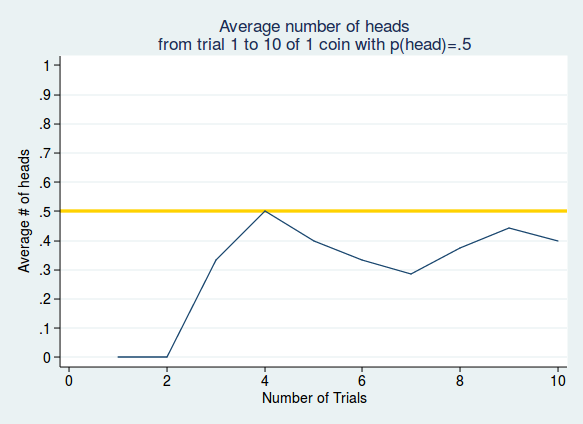
\includegraphics[scale=0.50]{coin_sim_10_fair.png}
\caption{Simulation w/ fair coin - n = 10}
\label{f1}
\end{figure}

	\begin{verbatim}
	 * toss 100 a fair coin
	 heads, flips(100)
	\end{verbatim}

See Figure~\ref{f2}\\

\begin{figure}[htp]
\centering
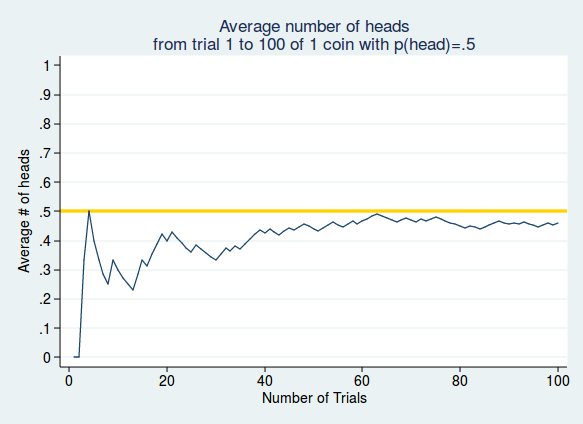
\includegraphics[scale=0.50]{coin_sim_100_fair.png}
\caption{Simulation w/ fair coin - n = 100}
\label{f2}
\end{figure}
	 
	\begin{verbatim}
	 * toss 1000 a fair coin
	 heads, flips(1000)
	\end{verbatim}

See Figure~\ref{f3}\\

\begin{figure}[htp]
\centering
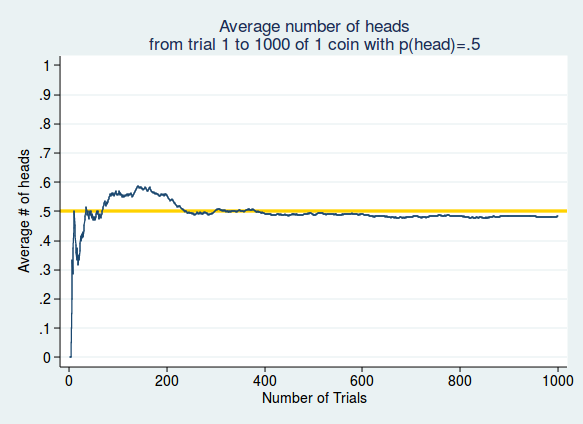
\includegraphics[scale=0.50]{coin_sim_1000_fair.png}
\caption{Simulation w/ fair coin - n = 1000}
\label{f3}
\end{figure}
	
	 
Try yourself with 1000000 coin tosses:
	 
	\begin{verbatim}
	 * toss 1000000 a fair coin
	 heads, flips(1000000)
	\end{verbatim}
	
	What if we use a biased coin?

	\begin{verbatim}
	 * toss 100 a biased coin w/ P(Head) = 0.3
	heads, flips(100) prob(.3)	 
	\end{verbatim}

See Figure~\ref{f4}\\

\begin{figure}[htp]
\centering
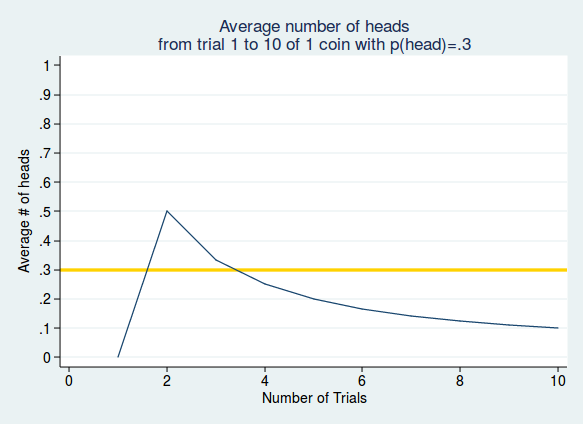
\includegraphics[scale=0.50]{coin_sim_10_biased.png}
\caption{Simulation w/ biased coin - n = 10}
\label{f4}
\end{figure}
	
	\begin{verbatim}
	 * toss 1000 a biased coin w/ P(Head) = 0.3
	heads, flips(1000) prob(.3)	 
	\end{verbatim}

See Figure~\ref{f5}\\

\begin{figure}[htp]
\centering
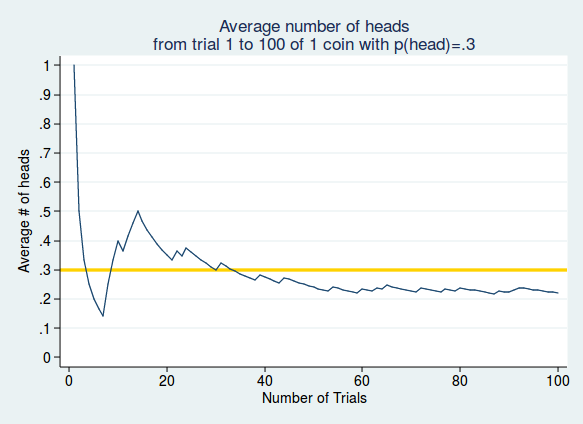
\includegraphics[scale=0.50]{coin_sim_100_biased.png}
\caption{Simulation w/ biased coin - n = 100}
\label{f5}
\end{figure}


\end{document}